\chapter{A Path to the Mass Gap}\label{ch:path}

Chapter~\ref{ch:theta} completed the toolkit. This chapter opens Part V, on the open problems. It assembles the pieces into a programme, separates what is done from what is not, and describes the idea we would try first on the rest. The first sections list the stages of the path and the open problems; Section~\ref{ch:isthere} states the mass gap conjecture in Thorin form and weighs the routes to the missing step; Section~\ref{ch:missing} lists ideas we have not used and recent work of others; Section~\ref{ch:threed} makes the case for attempting three dimensions first.

\section{The five stages}

\begin{enumerate}
\item[(i)] Positivity at every scale. Done for the lattice theory and for the Migdal Kadanoff rungs, not shown for a block spin transformation of the true flow. Reflection positivity on the lattice (Chapter~\ref{ch:positivity}), the preservation of nonnegative character coefficients at every Migdal Kadanoff rung (Lemma~\ref{lem:posB}), and the equivalence theorem (Theorem~\ref{thm:equivB}), which turns a uniform gap into a uniform inequality between positive Thorin densities with constant one.
\item[(ii)] Strong coupling. Done. The Osterwalder and Seiler cluster expansion~\cite{OSe} gives a positive lattice mass for $\beta<\beta_0$ (Chapter~\ref{ch:strong}), as does the log Sobolev argument of Shen, Zhu and Zhu~\cite{SZZ}.
\item[(iii)] The renormalization ladder in the Migdal Kadanoff approximation. Partly done. The asymptotics (Remarks~\ref{prop:decrementB} and~\ref{prop:sunB}), the monotonicity (Lemma~\ref{lem:mlrB}) and the covering on $[0.3,300]$ (Remark~\ref{prop:coverB}) are in place. The likelihood ratio hypothesis of the lemma is now a theorem (Corollary~\ref{cor:mlrall}). The decrement inequality for the heat kernel projected map is now Corollary~\ref{cor:contracts}; for the exact ladder the decimation half is open. Chapter~\ref{ch:strong} proves the first passage criterion for the projected map only. A computer assisted gap theorem for the Migdal Kadanoff hierarchical lattice, with asymptotic freedom scaling and an explicit coefficient, would follow if three things were added, each still open: a proof that the projected map controls the exact hierarchical recursion, a strong coupling mass with explicit constants, and boundedness in physical units (conditions (C), (D) and (E) of that chapter, where (E) fails as stated for the ladder and must be replaced), together with interval arithmetic and an explicit remainder for the rate. Confinement on hierarchical lattices of this type was proved by Ito in 1985~\cite{Ito85}; the new content would be the quantitative spectral statement and the identification of the coefficient as $(1-b^{-2})\E S_{\mathrm{BPY}}$.
\item[(iv)] Comparison with $\Z^4$. Open. The true renormalization flow must be bracketed between Migdal Kadanoff type flows strongly enough that the decrement inequality, or the uniform Thorin gap inequality, passes from the bracketing flows to the true one.
\item[(v)] The continuum theory. Announced, not independently checked. OpenAI announced on 26 October 2026 a proof, with a Lean formalisation, of the existence of certain four dimensional gauge theories including pure Yang Mills~\cite{OAI}; a review group led by D. Gross endorsed the existence part on 9 November. It is not refereed, and Woit disputes it as a weak existence result obtained by compactness~\cite{Woit26}. The announcement does not claim the mass gap. If the result is sustained it would supply a continuum theory, which is what this stage assumes. Ba\l aban's renormalization group~\cite{Ba87} controls the ultraviolet, and Magnen, Rivasseau and S\'eneor constructed SU(2) Yang Mills in finite volume~\cite{MRS}. What stage (v) still needs from us is the identification of the continuum spectral measures as weak limits of the lattice ones, so that Corollary~\ref{cor:continuumB} applies.
\end{enumerate}

Even if stage (iv) were established, stage (iii) would still need its remainder and its conditions, and stage (v) its identification of limits. Stage (iv) is where a new idea is needed.

\section{Why the comparison is hard}

Kadanoff's original argument~\cite{Ka75,Ka76} shows that bond moving\index{bond moving} gives one sided inequalities for free energies: moving bonds in one direction raises the free energy and in the other lowers it. Tomboulis\index{Tomboulis, E. T.}, in 2007~\cite{To07}, tried to use such inequalities to bracket the partition functions of the true theory in the presence of a centre vortex flux between those of Migdal Kadanoff\index{Migdal Kadanoff recursion} type flows, as a route to confinement\index{confinement} at all couplings. Ito\index{Ito, K. R.} and Seiler pointed out missing links in the argument, in a note of November 2007 and a longer discussion of March 2008~\cite{IS}, and Seiler gave a further critical discussion at the Confinement VIII conference~\cite{Se12}. The argument is not accepted as a proof.

The difficulty, in the language of this book, is a mismatch of objects. Free energies are logarithms of partition functions, one number per volume. The gap is a property of spectral measure\index{spectral measure}s, which are infinite dimensional. A bracket on free energies controls the spectral measures only through their total mass, and says nothing about where they are supported. The equivalence theorem tells us exactly what must be bracketed instead: the family of Thorin densities, or equivalently the correlations at all Euclidean times, uniformly in the lattice spacing.

\section{A probabilistic sandwich}

\begin{problem}[Thorin sandwich]\label{op:sandwichB}
Construct maps $R_-\le R_+$ on positive definite class functions, of Migdal Kadanoff type, whose flows bracket the true four dimensional spectral measures in the sense of the uniform Thorin gap inequality. Then prove the decrement inequality for $R_-$.
\end{problem}

The ordering $R_-\le R_+$ needs a meaning, with larger meaning more disordered, that is stronger coupling. The verification of Section~\ref{ch:verification} suggests one: the likelihood ratio\index{likelihood ratio order} order on laws of the rotation angle, which drove the monotonicity of $R$. Our proposal for attacking the problem has three steps.

First, realise the true block spin transformation of lattice gauge theory and the Migdal Kadanoff step on a common probability space. Both act on random group elements: the true transformation integrates out interior links of a block with their exact conditional law, and the Migdal Kadanoff step replaces that conditional law by a product of independent copies followed by a convolution. Brownian motion\index{Brownian motion on SU(2)}s on SU(2) supply a natural common space, because the heat kernel\index{heat kernel} laws are the fixed forms of decimation\index{decimation}.

Second, compare the resulting laws of the block holonomy in the likelihood ratio order. The tools are those of Section~\ref{ch:toolkit}: likelihood ratio orders are preserved by products and by convolution with log concave kernels, which are exactly the two Migdal Kadanoff operations.

Third, control the failure of log concavity. On a flat space the Gaussian laws are log concave and the argument would close. On SU(2) the Haar density $\sin^2\theta$ and the curvature factor $\theta/\sin\theta$ break log concavity away from the identity. Positive curvature helps some inequalities: the Riemannian Pr\'ekopa Leindler (Borell Brascamp Lieb) inequality of Cordero Erausquin, McCann and Schmuckenschl\"ager~\cite{CMS} holds on manifolds with Ricci curvature bounded below, and the Bakry \'Emery curvature dimension calculus~\cite{BE} gives functional inequalities for heat flow. Neither states that geodesic log concavity is preserved by heat flow or by marginalisation, and on the compact three sphere it could not be the right notion for laws spread over the group: a geodesically log concave function on the whole group is constant, as one sees by restricting it to a closed great circle. So at the crossover, where the laws are spread over the whole group, a substitute for geodesic log concavity is needed, and finding one is the concrete question. Chapter~\ref{ch:progress} adds one fact: in the variable $c=\cos\theta$ the heat kernel, and every power of it, is log concave on $[-1,1]$ (Corollary~\ref{cor:logconc}). The Haar weight $\sqrt{1-c^2}$ is also log concave in $c$, so the law of $c$ is log concave. The failure of log concavity is therefore a feature of the angle coordinate, and whether the likelihood ratio comparison can be carried out in the coordinate $c$ is open.

\section{Block spin transformations}

To make stage (iv) concrete we need a definition of the true renormalization step on $\Z^4$. The classical choice, used by Ba\l aban\index{Balaban, T.@Ba\l aban, T.}, is a block spin transformation. The lattice is partitioned into blocks of side $b$; for each pair of neighbouring blocks a new link variable is defined as an average of the products of original links along the paths that connect the block centres; and the new measure is the conditional law of these averaged variables, or a smoothed version of it with a Gaussian like kernel that keeps it concentrated near the average. Gauge invariance is preserved because the averaging is covariant.

Three features of this construction matter for a probabilistic comparison.
\begin{enumerate}
\item[(i)] The new link variables are functions of many old ones, and the new plaquette weight is no longer a function of single plaquettes: the effective action contains larger loops. Migdal Kadanoff truncates these to single plaquettes. A comparison must control the truncated terms, or show that they enter with a definite sign in the relevant order.
\item[(ii)] At weak coupling the block spin conditional laws are close to Gaussian on the Lie algebra, with corrections controlled by perturbation theory. In this regime Ba\l aban's bounds are available, and the comparison with Migdal Kadanoff should reduce to a comparison of the curvature corrections, which Section~\ref{ch:mk} expresses through the Biane Pitman Yor variable~\cite{BPY}.
\item[(iii)] At the crossover the laws spread over the whole group and no expansion applies. This is where the likelihood ratio and curvature tools must do their work, and where the positivity preserved at every rung (Lemma~\ref{lem:posB}) is essential, since it is the only structure that survives without an expansion.
\end{enumerate}

\section{A check in two and three dimensions}

In two dimensions Migdal Kadanoff is exact, because bond moving is trivial when $d-2=0$, and the comparison of stage (iv) holds with equality. The two dimensional theorem of Chapter~\ref{ch:twod} is therefore the complete version of the programme in that dimension. In three dimensions the coupling has dimension of mass, the theory is superrenormalizable, and Remark~\ref{prop:decrementB} shows that the precision falls by a factor $b$ per step even in flat space. There the gap is expected to follow from the dimensional running alone, and the curvature correction is subleading. A full comparison in three dimensions, between the Migdal Kadanoff ladder and the true lattice theory, would be a natural intermediate goal before four dimensions, and would test the probabilistic sandwich where the analytic stakes are lower.

\section{What a proof would have to contain}

It is useful to list what a complete argument along these lines would have to contain, so that progress can be measured.
\begin{enumerate}
\item A precise block spin transformation on $\Z^4$ for which the true flow is defined at every scale, together with reflection positivity at every scale.
\item Two Migdal Kadanoff type maps and a proof that they bracket the true flow in an order strong enough to control spectral measures.
\item A computer assisted proof of the decrement inequality for the lower map on a compact range of couplings, joined to the cluster expansion at strong coupling and to the asymptotic analysis at weak coupling (which needs an explicit remainder).
\item An identification of the continuum spectral measures with weak limits of the lattice ones, and an application of the continuum corollary.
\end{enumerate}
None of the four is done. Item 1 needs reflection positivity at every scale for the block spin transformation, for which we have no argument: Lemma~\ref{lem:posB} preserves nonnegative character coefficients at the Migdal Kadanoff rungs and does not give reflection positivity for the true flow. Item 3 presupposes the lower map of item 2, which does not yet exist. Item 4 is the identification of stage (v), still to be done. Item 2, the bracketing, is stage (iv) and is the problem.

\section{Open problems}

We collect the open problems of the book, in rough order of difficulty.

\begin{problem}\label{op:path1}
Bound the $O(1/\beta)$ remainder of Remark~\ref{prop:decrementB} explicitly using the variance of $S_{\mathrm{BPY}}$.
\end{problem}

\begin{problem}\label{op:path2}
Prove the likelihood ratio property of the SU(2) heat kernel analytically for all times, for instance from the image sum, and extend the monotonicity and covering\index{covering argument} arguments to SU(3).
\end{problem}

The SU(2) half of this problem is solved in Chapter~\ref{ch:progress}, by a product formula and not from the image sum. The SU(3) half is open.

\begin{problem}\label{op:path3}
Compute the next order of the Migdal Kadanoff decrement in terms of the cumulants of $S_{\mathrm{BPY}}$, and compare it with the two loop coefficient of the beta function.
\end{problem}

This problem is solved in Chapter~\ref{ch:progress}: Theorem~\ref{thm:expansion} gives the decrement in closed form, as the cumulant expansion of $S_{\mathrm{BPY}}$, with two loop ratio $1/(6b^2)$.

\begin{problem}\label{op:path4}
Build the Bayesian gap estimator of Chapter~\ref{ch:estimation} for published lattice glueball\index{glueball} correlators, and test the predictions of the Migdal Kadanoff ladder against them at intermediate couplings.
\end{problem}

\begin{problem}\label{op:path5}
Prove the uniform Thorin gap inequality at strong coupling with explicit constants, directly from the cluster expansion\index{cluster expansion}, and extend it as far as possible toward the crossover.
\end{problem}

\begin{problem}\label{op:path6}
Solve open problem~\ref{op:sandwichB}.
\end{problem}

\section{Closing}

In the Riemann programme the support of the measure is known and its positivity is the problem; in Yang Mills positivity is known and the support is the problem. Following the second problem has produced two dictionaries, an estimator, a two dimensional theorem, an identity linking Riemann's kernel to the three sphere, and a renormalization ladder whose running is the mean of a generalized gamma convolution. None of it proves the mass gap. It does place the remaining difficulty in one comparison between two flows of probability laws on a curved group.

The existence half of the problem was announced in 2026 as proved by a machine, with a Lean formalisation,~\cite{OAI}, endorsed by a review group and disputed by Woit~\cite{Woit26}. If the gap falls the same way, we expect the proof to contain, in some form, a statement about the supports of positive measures uniform across scales.

\section{Is There a Path to the Mass Gap?}\label{ch:isthere}\index{mass gap!conjecture in Thorin form}\index{roadmap}

This section states the mass gap conjecture in the form the book has reached, weighs the routes to the missing step of the path against each other, and says what we would try first.

\subsection{The conjecture in Thorin form}

Combining the equivalence theorem of Section~\ref{ch:routeB} with the existence of the continuum theory, if the 2026 announcement is sustained, the Clay mass gap for SU(2) would follow from the following, once stage (v) above, the identification of continuum spectral measures as weak limits of lattice ones, is done.

\begin{quote}
\textsc{Conjecture.} There is $\Delta_0>0$ such that for every gauge invariant observable $O$ and every lattice spacing $a$ along the renormalized trajectory, the Route B Thorin densities of $O$ in physical units satisfy $T^{(a)}_\alpha(z)\le e^{-\Delta_0(\alpha-\alpha')}T^{(a)}_{\alpha'}(z)$ for all $z$ and all $\alpha\ge\alpha'>\alpha_0$, where the spectral measures $\mu^{(a)}$ of $O$ satisfy $\sup_a\int e^{-\alpha_0E}\mu^{(a)}(\mathrm dE)<\infty$.
\end{quote}

By the same theorem this is equivalent to a uniform spectral gap and to uniform exponential decay of correlations. A uniform logarithmic Sobolev inequality for local dynamics measured in physical units (Section~\ref{ch:dynamic}) would imply it if the spin system equivalences of route B below extend to gauge theory, which is not shown; we do not know the converse. The conjecture implies the Clay problem for SU(2) once stage (v) is done, and the converse is not argued here. The reformulation changes the language, not the difficulty.

\subsection{The path at a glance}

\begin{figure}[t]
\centering
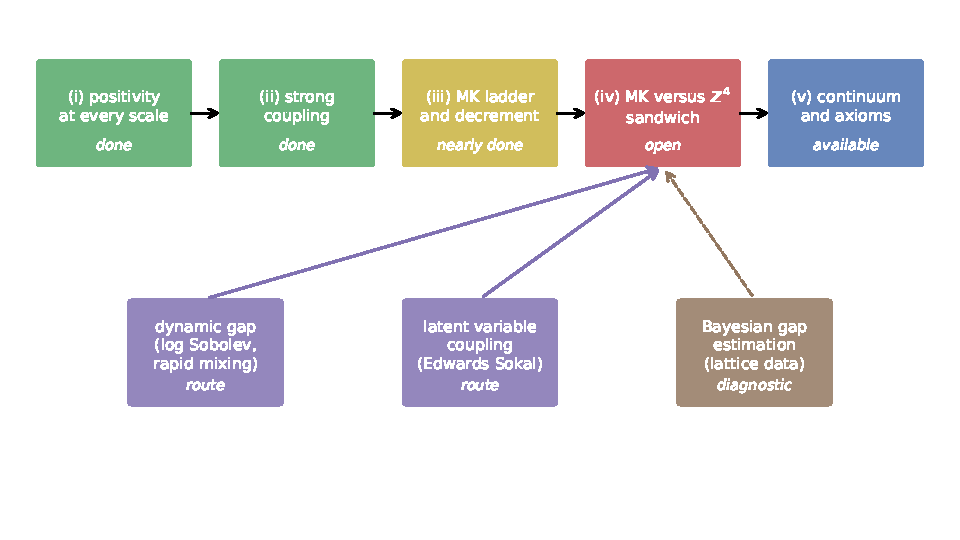
\includegraphics[width=\textwidth]{figures/roadmap.pdf}
\caption[A roadmap to the mass gap]{The five stages of the main path (top), colour coded by status, and three supporting routes (bottom): the dynamic gap through log Sobolev inequalities, a latent variable coupling in the style of Edwards and Sokal, and Bayesian gap estimation as a diagnostic.}
\label{fig:roadmap}
\end{figure}

The five stages of the path are those listed at the start of this chapter, and Figure~\ref{fig:roadmap} shows them with their status. Stage (iv), the comparison with $\Z^4$, is the step the next section is about.

\subsection{Three ways to attack stage (iv)}

\subsubsection*{A. A Thorin sandwich}
Bracket the true spectral measures directly. Its advantage is that the target statement is exactly the equivalence theorem; its weakness is that spectral measures are global objects and no local inequality is known to control them.

\subsubsection*{B. A dynamic sandwich}
Bracket Dirichlet forms of local dynamics along the ladder, and use the Stroock and Zegarlinski and Martinelli and Olivieri equivalences~\cite{SZ92,MO94} to convert a uniform log Sobolev inequality into a mass gap, which those equivalences give for finite range spin systems and which would have to be shown for gauge theory. Its advantage is that comparisons of Dirichlet forms are local and composable, and that the strong coupling end is already done by Shen, Zhu and Zhu~\cite{SZZ}. Its weakness is that log Sobolev constants are not known to behave monotonically under block spin transformations at weak coupling.

\subsubsection*{C. A latent variable coupling}
Realise the true block step and the Migdal Kadanoff step on one probability space, in the manner of Edwards and Sokal~\cite{ES88}, with latent variables chosen so that the plaquette laws are compared in the likelihood ratio order. Its advantage is that likelihood ratio orders are preserved by the two operations of the ladder when the kernels are log concave. Its weakness is that the Haar curvature breaks log concavity away from the identity; the Riemannian Pr\'ekopa Leindler inequality and Bakry \'Emery curvature on the three sphere are the tools one would try for it, although neither is known to give what is needed.

Our own preference is to try C first, then B, because they are local and because the probabilistic toolkit of this book is built for them. A is the cleanest statement and the hardest to attack directly.

\subsection{What would count as progress}

A complete proof is not the only useful outcome. In rough order of difficulty:
\begin{enumerate}
\item A rigorous, computer assisted version of stage (iii), giving an explicit gap function on hierarchical lattices for SU(2) and SU(3).
\item A comparison theorem in three dimensions, where the coupling is relevant rather than marginal and the stakes are lower.
\item A comparison theorem in four dimensions for a modified lattice action designed to make the comparison easier, for example with heat kernel plaquettes and a block spin rule adapted to Migdal Kadanoff.
\item A test of the Migdal Kadanoff predictions against published lattice glueball masses at intermediate coupling, by the estimator of Chapter~\ref{ch:estimation}.
\item The full comparison for the Wilson action.
\end{enumerate}

\subsection{Honest odds}

The mass gap has resisted fifty years of effort by people who knew more physics than we do. The approaches that came closest, Ba\l aban's renormalization group and Tomboulis's Migdal Kadanoff bracketing, both aim at the crossover between weak and strong coupling; the first stopped there and the second is not accepted as a proof. Our contribution is to put that crossover into a language, positive measures, Thorin densities, likelihood ratio orders, products and convolutions of laws on a curved group, in which probabilists have powerful tools, and to show by an exact result in two dimensions and by ladder computations that the language captures the mechanism. Whether the tools are strong enough for stage (iv) is unknown. We think the attempt is worth making, and the book is written so that others can make it.

\section{What We Might Be Missing}\label{ch:missing}\index{centre vortices}\index{gradient flow}\index{resurgence}\index{holography}

A book that proposes a route to an open problem should say which roads it has not taken. This section lists ideas from the physics and mathematics of gauge theory that we have not used, and for each says how it might bear on the approach of this book. It begins with recent work of others.

\subsection{Recent work of others}

Several recent results on lattice and continuum Yang Mills are close to our subject, though none is a mass gap for four dimensional Yang Mills at all couplings. On the lattice, Adhikari and Cao proved correlation decay for finite gauge groups at weak coupling~\cite{AC}; Cao, Park and Sheffield gave a random surface representation of lattice Yang Mills~\cite{CPS25}; and Cao, Nissim and Sheffield enlarged the regimes in which an area law is known, and gave a dynamical approach to it~\cite{CNS25}. In the continuum, the Yang Mills heat flow with random initial data~\cite{CC23} and stochastic quantisation have made progress in low dimensions: the Langevin dynamic of two dimensional Yang Mills~\cite{CCHS,ChSh23,BC23}, the local in time Langevin dynamic of three dimensional Yang Mills Higgs~\cite{CCHS3}, and, in two dimensions, the abelian Higgs equations~\cite{BC24} and the non abelian Yang Mills Higgs measure~\cite{BCHZ}. Chatterjee's survey~\cite{Ch19} is the place to start. These results concern finite groups at weak coupling, strong coupling, exact representations, lower dimensions, or a Higgs field, and the Thorin comparison of stage (iv) is not among them. The 2026 announcement of an existence proof for four dimensional Yang Mills~\cite{OAI,Woit26} is described in Section~\ref{sec:existence2026}.

\subsection{Centre vortices and 't Hooft's order parameters}

't Hooft~\cite{tH78} introduced the vortex free energy and the classification of phases of gauge theories by the behaviour of Wilson and 't Hooft loops. Mack and Petkova~\cite{MP80} gave a sufficient condition for confinement in terms of the free energy of a centre vortex, and Tomboulis's attempted proof~\cite{To07} used exactly this quantity, bracketing the twisted partition function between Migdal Kadanoff type bounds. Centre vortices are natural latent variables for the gauge field, and a latent representation built on them might supply the monotone coupling that Section~\ref{ch:isthere} asks for. We have not pursued this.

\subsection{Monopoles and dual superconductivity}

In three dimensional compact U(1), confinement is caused by monopoles, and G\"opfert and Mack~\cite{GM82} turned that into a theorem. In supersymmetric gauge theories Seiberg and Witten~\cite{SW94} showed that confinement follows from monopole condensation, the dual superconductor picture of Mandelstam~\cite{Ma76} and 't Hooft. No such mechanism has been established for pure nonabelian Yang Mills, but abelian projection and monopole condensation are widely studied on the lattice. A Thorin version of the G\"opfert and Mack argument, with the Coulomb gas of monopoles as the latent variables, is a direction we have not explored.

\subsection{Gradient flow}

L\"uscher's Yang Mills gradient flow~\cite{Lu10} smooths gauge fields along the gradient of the action. Observables at positive flow time are finite without renormalization, and the flow defines a scale. Flowed observables are the natural regularised operators for the offset measures of Chapter~\ref{ch:positivity}, and the flow itself is a deterministic renormalization map, close in spirit to the heat kernel convolution of the Migdal Kadanoff ladder. A comparison between the gradient flow and the ladder would make stage (iv) more concrete.

\subsection{Resurgence and renormalons}

The perturbative series of Yang Mills is not Borel summable, because of renormalons; Section~\ref{ch:sokal} discusses Borel summability. The theory of resurgence aims to reconstruct nonperturbative quantities from the large order behaviour of perturbation theory together with semiclassical saddles. The mass gap, of order $\Lambda$, is exactly such a quantity. We have not tried to connect resurgence with the Thorin structure, although Borel transforms and Laplace transforms of positive measures are close relatives.

\subsection{Holography}

The gauge gravity correspondence gives models of confining theories whose glueball spectra are computed from normal modes of fields in a curved higher dimensional geometry, as Witten and others showed in 1998~\cite{Wi98}. The spectral problem there is a Sturm Liouville problem, whose spectral measures are discrete and positive, and the gap is the lowest eigenvalue of a differential operator. These models are not pure Yang Mills, but they are caricatures in Kac's sense in which the gap is computable.

\subsection{Hamiltonian lattice gauge theory and quantum computation}

Kogut and Susskind's Hamiltonian formulation~\cite{KS75} puts the gauge theory on a spatial lattice with continuous time. The gap is then the gap of an explicit operator on a Hilbert space spanned by spin networks, the representation labels of Section~\ref{ch:latent}. Tensor network methods and quantum simulation target this formulation directly. The positivity of the transfer matrix is replaced by the self adjointness of the Hamiltonian, and the question becomes a spectral gap problem for a quantum many body system, where techniques such as the detectability lemma and martingale methods for frustration free Hamiltonians exist.

\subsection{Formal verification}

The existence proof announced in 2026 comes with a Lean formalisation~\cite{OAI}. Any proof of the mass gap will be long, multiscale, and partly computer assisted, and its credibility will depend on formal verification. Stage (iii) of the path, a computer assisted version of the gap statement on hierarchical lattices, is a natural first target for formalisation once its conditions are proved: it involves explicit special functions, interval arithmetic, and a monotone covering argument.

\subsection{Things we missed and have since found}

Some of what later chapters contain belongs under this title. We record five items here, because each changed our view of the problem, and at least one of them corrects a mistake.

\subsubsection*{Classical loop inequalities}
We listed $W_{12}\ge W_{11}^2$ as an open problem for nonabelian groups and tested it by simulation at eleven couplings. It is a three line consequence of reflection positivity for every compact group (Theorem~\ref{thm:doubling}). The lesson is general: reflection positivity gives a positive inner product, and every Schwarz inequality in it is a theorem about Wilson loops. The literature of the late 1970s and 1980s contains many, among them the convexity of the static potential and upper bounds on the string tension. Before posing a comparison as a conjecture one should ask whether it is a Schwarz or chessboard inequality.

\subsubsection*{The abelian control}
Any argument for confinement at weak coupling must fail for compact U(1) in four dimensions, where Guth~\cite{Gu80}, and Fr\"ohlich and Spencer~\cite{FS82}, proved that there is a massless Coulomb phase. This is the sharpest test of a proposed mechanism, and we had not applied it to the ladder. Doing so is instructive (Figure~\ref{fig:u1ladder}). On U(1) the heat kernel is a wrapped Gaussian, the group is flat, and bond moving maps the family to itself up to the images: the decrement of the ladder is not $\frac14$ but exponentially small, about $2\times10^{-5}$ at $\beta=1$, $4\times10^{-11}$ at $\beta=2$ and $2\times10^{-23}$ at $\beta=4$. So the ladder separates abelian from nonabelian theories by the mechanism this book has emphasised: no curvature, no running. But it does not produce a Coulomb phase. The decrement is positive, the flow still reaches strong coupling after a number of steps that grows exponentially in $\beta$, and the ladder predicts confinement with an astronomically large correlation length, which is false. The Migdal Kadanoff recursion is known to behave this way at a lower critical dimension. For the comparison problem the consequence is concrete: for U(1) the lower bracket must be a map with a line of fixed points, so no pair of brackets that both have positive decrement can be valid for all compact groups. A proof of the sandwich must use nonabelian structure, and the product formula and the curvature terms of Theorem~\ref{thm:expansionN} are where it enters.

\begin{figure}[t]
\centering
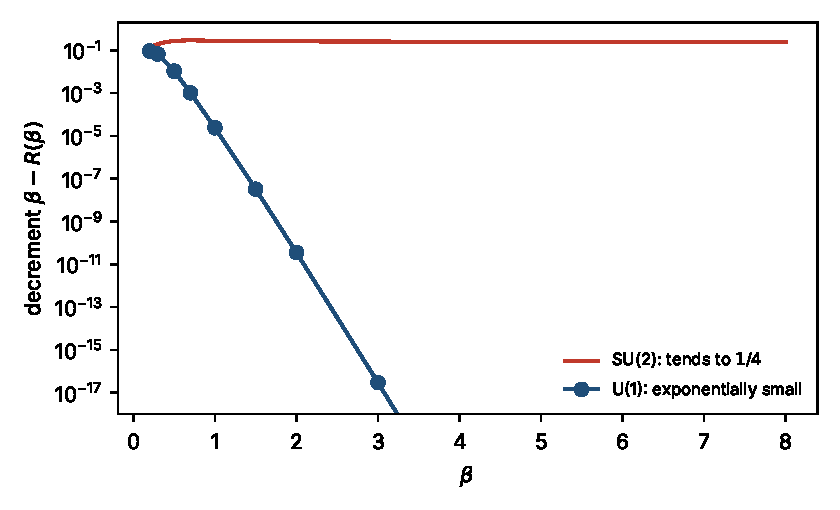
\includegraphics[width=0.8\textwidth]{figures/u1_ladder.pdf}
\caption[The abelian control: the ladder for U(1) and SU(2)]{The decrement $\beta-R(\beta)$ of the Migdal Kadanoff ladder in four dimensions with $b=2$, for SU(2), where it tends to $\frac14$, and for compact U(1) with heat kernel laws, where it is exponentially small in $\beta$.}
\label{fig:u1ladder}
\end{figure}

\subsubsection*{The centre, the antipode and the crossover}
Three known phenomena sit in the window of couplings where our methods are weakest, and we had not connected them. The first is the phase structure in the plane of fundamental and adjoint couplings found by Bhanot and Creutz~\cite{BC81}: an action with an adjoint term has first order transitions, driven by the centre element $-1$ and its $\Z_2$ monopoles, on lines that end at a critical point close to the Wilson axis. The rapid crossover of the Wilson theory near $\beta=2.2$, and the failure of asymptotic scaling there, are usually attributed to that nearby endpoint. The second is the roughening transition of the strong coupling expansion near $\beta=1.9$, beyond which the series for the string tension cannot be continued. The third is our own bad cap at the antipode (Theorem~\ref{thm:hemisphere}), which is the same centre element seen in the convolution kernel, and whose mass peaks at $\beta\approx0.8$ in the ladder's coordinate, roughly $\beta\approx2.2$ after the shift of $1.45$ found in Chapter~\ref{ch:progress}. The ladder acts on whole plaquette laws, so it has an adjoint coupling, the coefficient $u_3$; following the flow in the plane $(u_2,u_3)$ against the Bhanot and Creutz diagram, and repeating the tests of Chapter~\ref{ch:progress} for the heat kernel and positive plaquette actions, which were designed to remove the centre artefacts, is a computation we have not done.

\subsubsection*{Finite temperature and our small lattices}
A periodic lattice of temporal extent $N_t$ is a system at temperature $1/(N_ta)$, and SU(2) deconfines above a critical coupling: $\beta_c=2.30$ for $N_t=4$ and $2.51$ for $N_t=8$~\cite{FHK}. Our $8^4$ runs at $\beta\ge3$ and all our $4^4$ runs above $\beta=2.3$ are therefore in small, hot boxes, not in the confined phase of the infinite lattice. For the quantities we measured this is harmless and in one case intended: plaquettes and $2\times2$ loops are local, their finite size corrections are small, and the agreement with the perturbative values tabulated for Conjecture~\ref{prop:weaksandwich}, computed on the same $8^4$ lattice, confirms it; the matching of Section~\ref{ch:plgbc} compares two lattices of the same physical size by design. But no string tension or glueball mass could be extracted from those runs, and the text should not be read as if it could. The deconfinement transition is also a subject we have left out: the Polyakov loop, centre symmetry and the Svetitsky and Yaffe universality argument~\cite{SY82} give a second, well understood order parameter for confinement.

\subsubsection*{The Hamiltonian form}
Proposition~\ref{prop:groundstate} of Section~\ref{ch:h6ym} states the gap in terms of the Poincar\'e constant of the ground state measure. We had treated the Hamiltonian formulation only as a topic for quantum simulation. It deserves more: it is the form of the problem in which the gap is the spectral gap of a single diffusion.

\subsection{Loop equations and the bootstrap}

The Schwinger Dyson equations of lattice gauge theory, the Makeenko and Migdal loop equations~\cite{MM79}, relate the expectation of a Wilson loop to those of loops deformed by one plaquette. In the dictionary of Section~\ref{ch:dictionary} they are score equations. Chatterjee~\cite{Ch19so}, and Shen, Smith and Zhu, have derived and used them rigorously. In the last few years they have been combined with positivity into a numerical bootstrap: Anderson and Kruczenski~\cite{AK17}, and Kazakov and Zheng~\cite{KZ23}, impose the loop equations as linear constraints on a finite set of loop expectations and reflection positivity as the semidefiniteness of matrices of such expectations, and obtain rigorous two sided bounds on the plaquette that tighten as the set grows.

This is close to the present book and we have not used it. The semidefinite matrices of the bootstrap are the Hankel and Gram matrices of Chapter~\ref{ch:positivity}; Theorem~\ref{thm:doubling} is one of their two by two minors. The bootstrap is a systematic way to generate comparison inequalities of exactly the kind the sandwich needs, with a certificate. Two uses suggest themselves. A bootstrap bound on $W_{22}$ given $W_{11}$ would be a rigorous bracket to set beside the two caricatures. And a bootstrap on correlators at several time separations, with the gap as the variable, is the certified version of the estimator of Chapter~\ref{ch:estimation}: the largest $m$ for which a positive spectral measure supported on $[m,\infty)$ is consistent with the loop equations.

\subsection{Generalised symmetries}

Since the work of Gaiotto, Kapustin, Seiberg and Willett~\cite{GKSW}, confinement in pure gauge theory is described as the statement that a one form symmetry, the centre symmetry acting on Wilson loops, is unbroken: the area law is the disordered phase of that symmetry and the perimeter law its broken phase. Anomaly matching for this symmetry constrains the possible long distance behaviour, for instance at vacuum angle $\pi$. This language gives precise meaning to the order parameters of 't Hooft, organises the role of the centre that appears in several places above, and suggests that the right object for a comparison theorem is not the plaquette law alone but the pair consisting of the Wilson loop and the centre vortex free energy, which are dual under the symmetry. Tomboulis's attempted proof~\cite{To07} worked with that pair.

\subsection{Gauge fixed and functional methods}

A large physics literature approaches the gap through gauge fixed correlation functions: Gribov's restriction of the functional integral~\cite{Gr78}, Zwanziger's horizon condition, Cornwall's dynamically generated gluon mass, and functional renormalization group and Dyson Schwinger studies of the Landau gauge propagators, checked against lattice simulations in fixed gauges. These methods produce a mass scale in the gluon propagator. They are not rigorous, they work with quantities that are not gauge invariant and not reflection positive, and their relation to the gauge invariant spectral measures of this book is indirect. But they are the main source of quantitative intuition about how a mass arises at intermediate momenta, and a probabilistic reading of the Gribov region, as a constraint set of the kind met in slice sampling, may be worth having.

\subsection{Statistics we have not used}

Finally, two statistical ideas we have not developed. Empirical Bayes estimation of the spectral measure across many lattice spacings, borrowing strength along the renormalized trajectory, would sharpen the gap estimator of Chapter~\ref{ch:estimation}. And generative Bayesian computation, which learns a map from data to posterior through deep networks, could learn the renormalization map itself from simulations, giving an empirical version of the ladder against which the Migdal Kadanoff caricature could be compared.

\section{Three Dimensions First}\label{ch:threed}\index{three dimensions}\index{Karabali, D.!Kim, C. and Nair, V. P.}\index{Teper, M.}

The tests of Chapter~\ref{ch:progress} recommend three dimensions as the place to attempt the comparison step. This section says why, collects what is known there, and states the three dimensional version of the path.

\subsection{Why three dimensions is easier}

In three dimensions the gauge coupling $g^2$ has the dimension of mass. The theory is superrenormalizable: there is no logarithmic running, the coupling is relevant, and the lattice coupling $\beta=4/(ag^2)$ for SU(2) is simply proportional to the inverse lattice spacing. All masses are multiples of $g^2$, and the continuum limit is $\beta\to\infty$ with $a=4/(\beta g^2)$.

For the ladder this changes everything that was delicate in four dimensions. The Gaussian ledger of Section~\ref{ch:mk} gives, per step of scale factor $b$,
\[
\frac1{t''}=\frac{b^{-1}}{t}-\frac{(b-1)\,\E S_{\mathrm{BPY}}}{2b^2}+O(t),
\]
so the inverse coupling $1/t$ is divided by $b$ at every step whatever the curvature term does, and the number of steps to strong coupling is $\log_b\beta$ up to a constant. The scale is set by counting, not by an exponentially sensitive crossover. An error in the curvature term changes the answer by a factor near one, not by a factor of fifty.

\subsection{What is known}

Ultraviolet stability in three dimensions is part of Ba\l aban's programme and is simpler than in four. The mass gap is open in three dimensions too: no proof of confinement or of a gap exists for the nonabelian theory at weak lattice coupling. For compact U(1) in three dimensions, G\"opfert and Mack~\cite{GM82} proved confinement and a mass gap at all couplings, by the monopole gas. Numerically the theory is known to high precision: Teper's simulations~\cite{Te99} give $\sqrt\sigma/g^2=0.3353$ for SU(2), with glueball masses in fixed ratio to $\sqrt\sigma$.

There is also an analytic prediction. Karabali, Kim and Nair~\cite{KKN}, working in the Hamiltonian formulation with gauge invariant matrix variables, obtained
\[
\sqrt\sigma=g^2\sqrt{\frac{N^2-1}{8\pi}},
\]
which is $0.3455\,g^2$ for SU(2), three percent above the lattice value. Their vacuum wave functional is, to leading order, Gaussian in the magnetic field with a kernel that has a gap, and the string tension is that of a two dimensional Yang Mills theory with an effective coupling. In the language of this book: the three dimensional vacuum, restricted to a plane, looks like a two dimensional heat kernel measure, the exactly solvable case of Chapter~\ref{ch:twod}.

\subsection{The ladder in three dimensions}

\begin{figure}[t]
\centering
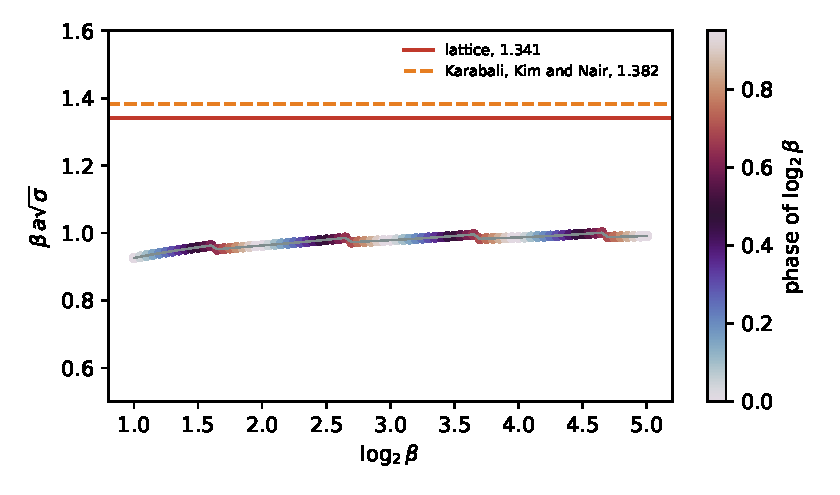
\includegraphics[width=0.9\textwidth]{figures/mk_3d.pdf}
\caption[The three dimensional ladder against lattice and analytic values]{The ladder's prediction of $\beta a\sqrt\sigma$ for three dimensional SU(2) as a function of $\log_2\beta$, coloured by the phase of $\log_2\beta$, against the lattice continuum value and the prediction of Karabali, Kim and Nair. The ladder is flat in $\log_2\beta$ at weak coupling to within two percent; the small remaining modulation is an artefact of the discrete scale factor.}
\label{fig:mk3d}
\end{figure}

With no fitted constant, the ladder with $b=2$ and Wilson start gives $\beta a\sqrt\sigma$ between $0.98$ and $1.00$ for $8\le\beta\le32$, with mean $0.99$ over a period of $\log_2\beta$ (Figure~\ref{fig:mk3d}; computed by \texttt{code/mk\_sigma.py}, run from \texttt{code/mk\_3d.py}). The lattice value is $1.341$ and the analytic prediction $1.382$. The ladder is low by twenty six percent on average. The remaining modulation, about two percent peak to peak, is an artefact of the discrete scale factor: the true theory has no preferred scale factor, and the modulation measures how much the answer depends on where the integer number of steps happens to end.

Twenty six percent is the size of bracket that a comparison theorem in three dimensions must tolerate. Since the conclusion sought is only that the string tension and the gap are positive multiples of $g^2$, and not their values, a bracket of that width is harmless.

\subsection{The sandwich in three dimensions}

Chapter~\ref{ch:sandwich} measured the laws of the $2\times2$ and $4\times4$ loops on a $16^3$ lattice. We collect the three dimensional numbers here, since they are the evidence for the problem below.

\begin{center}
\small
\begin{tabular}{ccccccc}
\toprule
 & \multicolumn{3}{c}{$u_2$ of the $2\times2$ loop} & \multicolumn{3}{c}{$u_2$ of the $4\times4$ loop} \\
$\beta$ & indep. & measured & MK & indep. & measured & MK \\ \midrule
4 & 0.281 & 0.323 & 0.540 & 0.0062 & 0.021 & 0.267 \\
6 & 0.463 & 0.522 & 0.686 & 0.046 & 0.126 & 0.456 \\
9 & 0.615 & 0.672 & 0.787 & 0.143 & 0.305 & 0.613 \\
14 & 0.739 & 0.785 & 0.862 & 0.298 & 0.494 & 0.740 \\
\bottomrule
\end{tabular}
\end{center}

At one step the two caricatures differ by a factor between $1.2$ and $1.9$, and the truth sits about a third of the way from the independent end. At two steps they differ by a factor between $2.5$ and $43$, and the truth is near the middle on a logarithmic scale. At weak coupling perturbation theory gives $\log W_{22}/\log W_{11}=3.120$ and $\log W_{44}/\log W_{11}=8.715$, against $4$ and $16$ for independent plaquettes and $2$ and $4$ for the ladder; the measured ratio at $\beta=14$ is $3.21$.

\subsection{The path in three dimensions}

\begin{enumerate}
\item[1.] Positivity. Reflection positivity on the lattice and the preservation of nonnegative character coefficients by the ladder hold in any dimension; reflection positivity for a block spin transformation of the true flow is not shown, as in four dimensions.
\item[2.] Strong coupling. The cluster expansion and the log Sobolev argument are not specific to four dimensions.
\item[3.] The ladder. In three dimensions the map $\beta\mapsto R_3(\beta)$ contracts at weak coupling by the factor $b$. The decrement inequality $R_3(\beta)<\beta$ is immediate there, and the covering argument is needed only on a bounded range near the crossover. Monotonicity is Corollary~\ref{cor:mlrall}, which does not depend on the dimension.
\item[4.] The comparison. The empirical sandwich of Chapter~\ref{ch:sandwich} holds in three dimensions at every coupling and scale we tried; there bond moving has power $b$ and not $b^2$, and the two caricatures are closer together. Because the flow is contracting, errors in a single step do not accumulate multiplicatively in the scale as they do when the coupling is marginal.
\item[5.] The continuum. Superrenormalizability makes the ultraviolet limit far simpler than in four dimensions.
\end{enumerate}

\begin{problem}\label{op:path7}
Prove that three dimensional SU(2) lattice gauge theory with the Wilson action has a mass gap $m(\beta)\ge c_0/\beta$ in lattice units for all $\beta$, with $c_0>0$, by bracketing one block spin step between two contracting Migdal Kadanoff type maps.
\end{problem}

This is the problem we would work on first. It is open, it is believed true, the exactly solvable two dimensional theory sits inside it through the Karabali, Kim and Nair picture, and every tool of this book applies without the marginal flow that makes four dimensions hard.

\section*{Exercises}
\begin{enumerate}
\item Derive the three dimensional ledger of Section~\ref{ch:threed} from the general formula of Section~\ref{ch:mk} and show that the number of steps to strong coupling is $\log_b\beta+O(1)$.
\item Show that a function of the form $\beta a\sqrt\sigma$ computed from a recursion with scale factor $b$ is asymptotically periodic in $\log_b\beta$ at weak coupling.
\item Compute the Karabali, Kim and Nair value of Section~\ref{ch:threed} for SU(3) and compare it with the lattice value $0.5530$.
\end{enumerate}
